\documentclass[11pt]{article}
\usepackage[margin=1in]{geometry}
\usepackage{amsmath,amssymb,booktabs,graphicx,setspace,caption,hyperref}
\usepackage[T1]{fontenc}
\usepackage{mathpazo}
\setlength{\parindent}{0pt}
\setlength{\parskip}{0.6em}
\captionsetup{font=small,skip=6pt}
\title{Panel MS-AR(1) after a common random-walk trend\\[0.4em]\large Seasonally adjusted real GDP per worker}
\author{}
\date{}
\begin{document}
\maketitle
\section{Model}
Two-step. Step 1 builds a \emph{common} trend from average growth of countries observed in consecutive quarters (not from the level mean, which falls when poorer countries enter). Log seasonally adjusted real GDP per worker, 2026-09-17 vintage, from 1987Q1 onward.
\begin{align}
\Delta\tau_t &= \frac{1}{n_t^{\mathrm{cont}}}\sum_{i\in C_t\cap C_{t-1}} (y_{it}-y_{i,t-1}), \\
\tau_t &= \tau_{t_0}+\sum_{s=t_0+1}^{t}\Delta\tau_s.
\end{align}
The level of $\tau$ is pinned to the balanced-core mean at $t_0$. Mean $\Delta\tau$ is 0.0045 per quarter (3 countries present in every quarter). Step 2 is estimated on $y_{it}^\ast=y_{it}-\hat\tau_t$, with no extra $gt$:
\begin{align}
y_{it}^\ast &= a_i + b_i\,\lambda^{t-T_{i0}} + z_{it}, \\
a_i &\sim \mathcal{N}(\alpha,\omega^2),\qquad b_i \sim \mathcal{N}(0,\omega_b^2) \ \text{independent}, \\
z_{i,t+1} &= \bigl(1-\rho(s_{it})\bigr)\mu(s_{it}) + \rho(s_{it})\, z_{it} + \sigma(s_{it})\,\varepsilon_{it}.
\end{align}
$\lambda=0.99$ is fixed. $|\rho|<0.99$. Three regimes; median $\mu$ pinned at 0; $\sigma$ and $\rho$ switch. $T_{i0}$ is country $i$'s first observation after filters. Random effects: 7$\times$7 Gauss--Hermite. Plotted cycles use posterior-mean $a_i$ and $b_i$. The common trend $\tau_t$ is discarded for the structural MS-AR. Standard errors ignore step-1 uncertainty.
\begin{figure}[h]
\centering
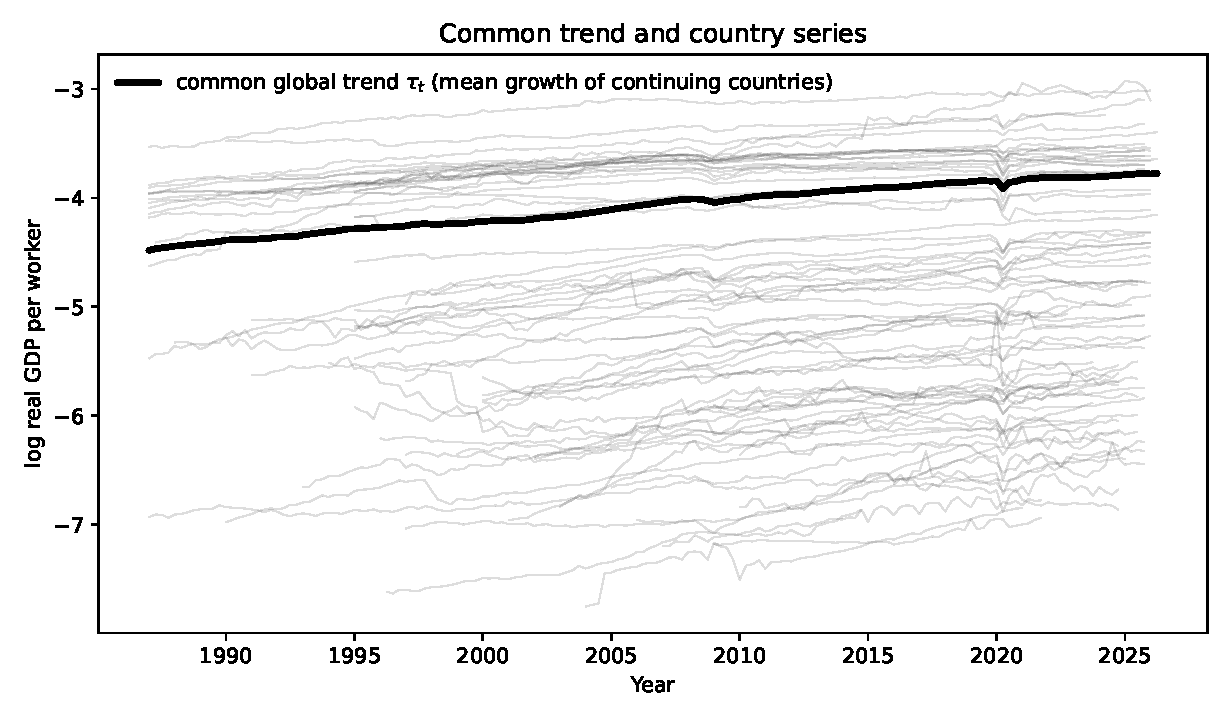
\includegraphics[width=0.88\textwidth]{figs/tau_rw.pdf}
\caption{Faint lines: country log real GDP per worker. Thick line: common $\tau_t$ from average growth of continuing countries (new entrants do not shift the level).}
\end{figure}
\clearpage
\section{Common RW trend removed; RE intercepts plus catch-up, lambda=0.99}
2026-09-17 SA panel, $y_{it}-\hat\tau_t$, from 1987. 74 countries, 8291 observations, 1987-Q1--2026-Q2. $|\rho|<0.99$, $\lambda=0.99$ fixed. Fitted countries: 74. Observations: 8291. Log-likelihood: 22666.61. Ergodic mean of the cycle $E[z]=0.0234$ (0.0221).
Permanent RE intercepts and catch-up $y_{it}=a_i + b_i\lambda^{t-T_{i0}}+z_{it}$ with $\alpha=-0.9515$ (0.0172), $\omega=0.6655$ (0.0124), $\lambda=0.9900$ (fixed), $\omega_b=0.5678$ (0.0123). Posterior-mean $a_i$: mean -1.104, min -3.191, max 0.584. Posterior-mean $b_i$: mean 0.011, min -1.303, max 1.343.
\begin{table}[h]
\centering
\caption{Regime AR(1), transition matrix, and ergodic $\pi$. Columns are regimes.}
\begin{tabular}{lccc}
\toprule
 & (0) & (1) & (2) \\
\midrule
$\mu$ & -0.6059 & 0.0000 & 0.1779 \\
 & (0.1485) & --- & (0.0411) \\ \addlinespace
$\sigma$ & 0.0721 & 0.0072 & 0.0187 \\
 & (0.0028) & (0.0001) & (0.0005) \\ \addlinespace
$\rho$ & 0.9899 & 0.9900 & 0.9900 \\
 & (0.0006) & (0.0000) & (0.0000) \\ \addlinespace
$\Pi_{0\cdot}$ & 0.6963 & 0.0005 & 0.3032 \\
 & (0.0354) &  & (0.0348) \\ \addlinespace
$\Pi_{1\cdot}$ & 0.0065 & 0.9467 & 0.0468 \\
 & (0.0026) & (0.0053) & (0.0058) \\ \addlinespace
$\Pi_{2\cdot}$ & 0.0533 & 0.0625 & 0.8842 \\
 & (0.0069) & (0.0072) & (0.0100) \\ \addlinespace
$\pi$ & 0.0845 & 0.4944 & 0.4211 \\
 & (0.0097) & (0.0255) & (0.0218) \\ \addlinespace
\bottomrule
\end{tabular}
\end{table}
\begin{figure}[h]
\centering
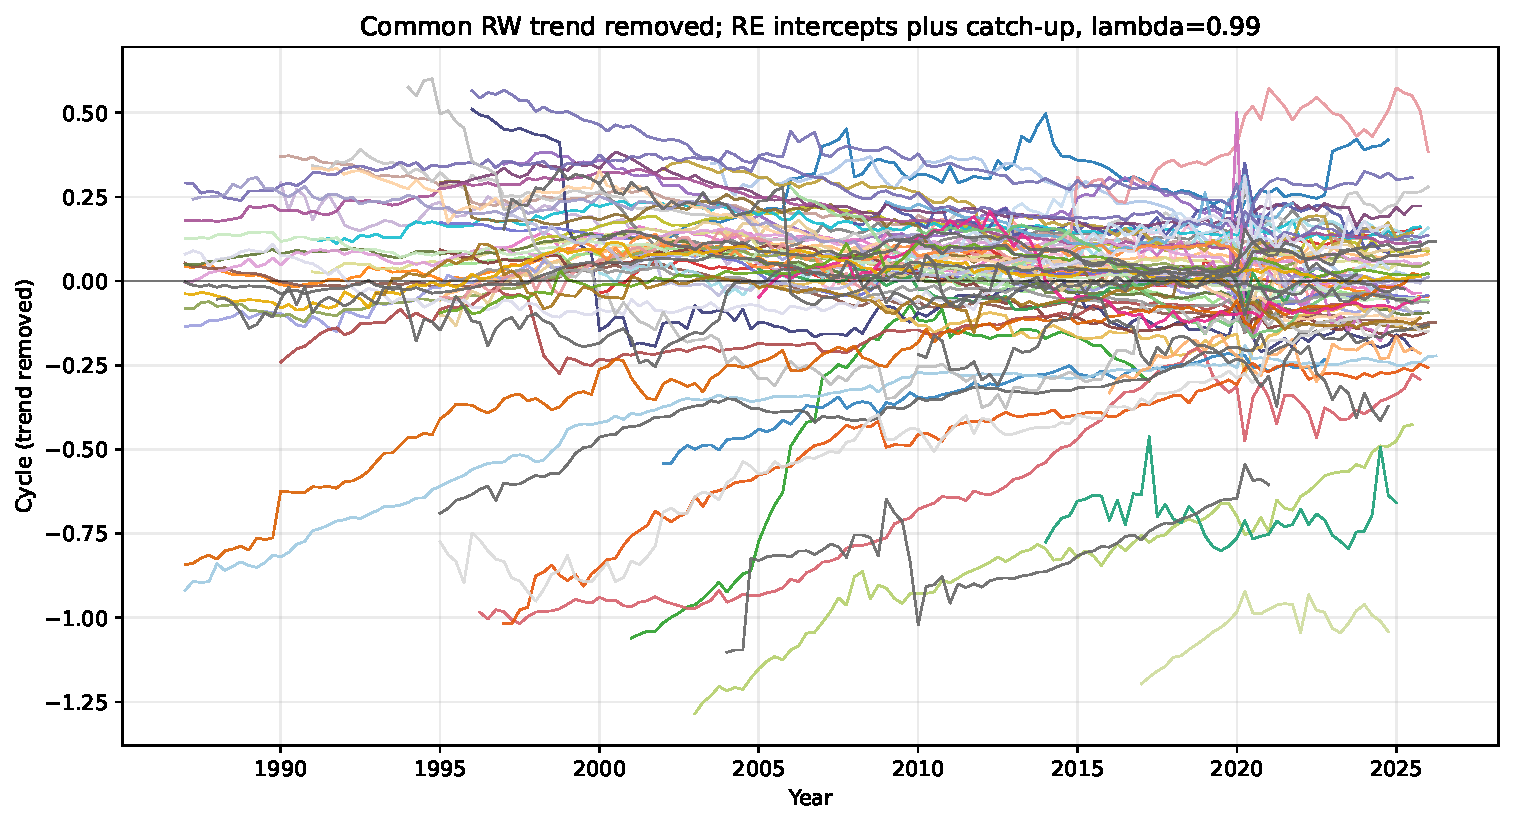
\includegraphics[width=0.75\textwidth]{figs/cycle_rw_lam99.pdf}
\caption{Country cycles after removing $\tau_t$, $a_i$, and $b_i\lambda^{t-T_{i0}}$.}
\end{figure}
\end{document}
